\documentclass[a4paper,10pt]{report}
\usepackage{amsmath, amsfonts, amssymb, physics}
\usepackage{revsymb}

\usepackage{amsmath,amsfonts,amsthm,physics,braket,indentfirst}
\usepackage{float}

\usepackage[a4paper,
            left=3cm,
            right=3cm,
            top=3cm,
            bottom=3cm]{geometry}

\usepackage{graphicx}

\usepackage{hyperref}
\hypersetup{
	colorlinks=true,       	
	linkcolor=blue,          	
	citecolor=blue,        		
	urlcolor=blue}
\usepackage{url}

\newtheorem{alg}{Algorithm}
\newtheorem{exe}{Exercise}

\title{PhD Thesis}
\author{M. Gil de Oliveira}
\date{\today}

\begin{document}

\maketitle

\chapter{Wave Optics}

\section{Propagation in free space}

Although we aim to study the propagation of light in turbulent media, it is important to first understand how light propagates in free space. This will provide us with a solid foundation for understanding the effects of turbulence on light propagation.

\subsection{The paraxial wave equation}

Our starting point will be the wave equation for the electric field, which is derived from Maxwell's equations. In free space, the wave equation can be expressed as
\begin{equation}
    \label{eq:wave equation}
    \nabla^2 E - \frac{1}{c^2} \partial_t^2 E = 0,
\end{equation}
where $E$ is the electric field, which we assumed to have a fixed polarization, $c$ is the speed of light in vacuum, and $\nabla^2$ is the Laplacian operator in three-dimensional space. 

A well known class of solutions are the plane waves $E(\mathbf{r}, t) = E_0 e^{i(\mathbf{k} \cdot \mathbf{r} - \omega t)}$ satisfies this equation, where $\mathbf{k}$ is the wave vector, $\omega$ is the frequency, and $E_0$ is a constant amplitude. The norm of the wave vector is related to the frequency $\omega$ by $ck = \omega$. These solutions have a well-defined direction of propagation defined by the wave vector $\mathbf{k}$, which we assume to be the $z$ direction, i.e., $\mathbf{k} = k \hat{\mathbf{z}}$.

Nonetheless, this class of solutions is nonphysical, as the electric field is not localized in space and contains an infinite amount of energy. A more physically relevant solution can be obtained by considering a field of the form
\begin{equation}
    E(\mathbf{r}, t) = u(\mathbf{r}) e^{i(kz - \omega t)},
\end{equation}
where $u(\mathbf{r})$ is a complex function describing an envelope that modulates the plane wave. By substituting this expression into the wave equation \eqref{eq:wave equation}, we obtain
\begin{equation}
    \nabla^2 u + 2ik \partial_z u= 0.
\end{equation}

\begin{figure}[h]
    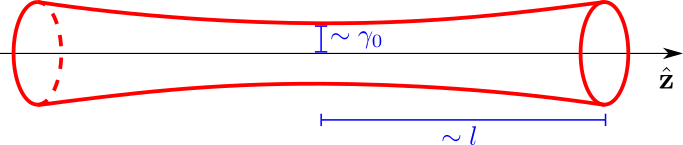
\includegraphics[scale=0.7]{images/feixe_paraxial.png}
    \centering
    \caption{Envelope of a paraxial beam.}
    \label{fig: paraxial beam}
\end{figure}

The typical envelope of a laser beam is shown in Fig. \ref{fig: paraxial beam}. The envelope $u(\mathbf{r})$ varies slowly along the $z$ direction. More precisely, the variation of $u$ in the $z$ is much smaller than the scale of variation defined by the wave number $k$. Therefore, we will assume that $\partial_z^2 u \ll k \partial_z u$, which allows us to neglect the second derivative with respect to $z$ in the wave equation. This leads us to the paraxial wave equation
\begin{equation}
\label{eq:paraxial}
    \nabla^2_T u + 2ik \partial_z u = 0,
\end{equation}
where $\nabla^2_T$ is the Laplacian operator restricted to the transverse plane, i.e., $\nabla^2_T = \partial_x^2 + \partial_y^2$.

\subsection{Solution of the paraxial wave equation}

The paraxial wave equation \eqref{eq:paraxial} is a partial differential equation that describes the propagation of light beams in the paraxial approximation. We want to find a solution for this equation, which will allow us to understand how light propagates in free space. In particular, we want to find a solution for the electric field envelope $u(x,y,z)$ given an initial condition $u(x,y,0)$ at $z=0$.

As it the equation is, the most straightforward way to solve it is to use the Fourier transform. Let us then define the Fourier transform of $u(x,y,z)$ as
\begin{equation}
\label{eq:fourier_transform}
    \tilde{u}(k_x, k_y,z) = \int_{\mathbb{R}^2} dx dy \ e^{-i(k_x x + k_y y)} u(x,y,z),
\end{equation}
which can be inverted as
\begin{equation}
\label{eq:inverse_fourier_transform}
    u(x,y,z) = \frac{1}{(2\pi)^2} \int_{\mathbb{R}^2} dk_x dk_y \ e^{i(k_x x + k_y y)} \tilde{u}(k_x, k_y,z).
\end{equation}
Substituting this expression into the paraxial wave equation \eqref{eq:paraxial}, we obtain
\begin{equation}
    \left( -k_x^2 - k_y^2 + 2ik \partial_z \right) \tilde{u}(k_x, k_y,z) = 0.
\end{equation}
This is a simple ordinary differential equation in $z$ for each fixed pair $(k_x, k_y)$. The solution can be written as
\begin{equation}
\label{eq:solution_paraxial_fourier}
    \tilde{u}(k_x, k_y,z) = \tilde{u}(k_x, k_y,0) e^{-i(k_x^2 + k_y^2)z/2k}.
\end{equation}

This provides a step-by-step algorithm for solving the paraxial wave equation:
\begin{alg}[Angular spectrum method]
\leavevmode
\begin{enumerate}
    \item Compute the Fourier transform $\tilde{u}(k_x, k_y,0)$ of the initial condition $u(x,y,0)$ using \eqref{eq:fourier_transform}.
    \item For each pair $(k_x, k_y)$, compute the solution $\tilde{u}(k_x, k_y,z)$ using the formula \eqref{eq:solution_paraxial_fourier}.
    \item Finally, compute the inverse Fourier transform to obtain the solution $u(x,y,z)$.
\end{enumerate}
\end{alg}

This is the angular spectrum method, which is a powerful technique for solving the paraxial wave equation. It allows us to compute the solution in the Fourier domain, where the equation becomes much simpler to solve. This is the basis for the method we will use to numerically simulate the propagation of light in turbulent media.

An equivalent way to express the solution of the paraxial equation, that is more simple from the analytical point of view, is obtained by substituting the expression \eqref{eq:solution_paraxial_fourier} into the inverse Fourier transform \eqref{eq:inverse_fourier_transform} and applying the convolution theorem. \footnote{This theorem states that the Fourier transform of convolution is the product of the Fourier transforms.} This leads to the following expression for the solution:
\begin{equation}
\label{eq:fresnel_diffraction}
    u(x,y,z) = \frac{k}{2\pi i z} \int_{\mathbb{R}^2} dx^\prime dy^\prime u(x^\prime,y^\prime,0) e^{ik\left[ (x-x^\prime)^2 + (y-y^\prime)^2 \right] / 2z}.
\end{equation}

This is the so-called Fresnel diffraction integral \cite{goodman2017introduction, schmidt2010numerical}.

\begin{exe}
    Apply the Fresnel diffraction integral to solve the paraxial wave equation for the initial condition
    \begin{equation}
        u(x,y,0) = e^{-(x^2+y^2)/w^2},
    \end{equation}
    where $w$ is a constant that defines the width of the beam (waist). 
\end{exe}

The Fresnel diffraction formula can be simplified when the distance $z$ is sufficiently large. In fact, assume that our initial condition $u(x,y,0)$ is mostly localized in a disk of radius $w$ around the origin, i.e., $u(x,y,0) \approx 0$ for $x^2+y^2 > w^2$. Then, when $z \gg kw^2/2$, the term $k[(x^\prime)^2 + (y^\prime)^2] / 2z$ in the exponent of \eqref{eq:fresnel_diffraction} does not contribute to the integral, and we can approximate the Fresnel diffraction integral as
\begin{equation}
    u(x,y,z) \approx \frac{k e^{ik\left( x^2 + y^2 \right) / 2z}}{2\pi i z} \int_{\mathbb{R}^2} dx^\prime dy^\prime u(x^\prime,y^\prime,0) e^{ik\left( xx^\prime + yy^\prime \right) / z}.
\end{equation}
This is known as the Fraunhofer diffraction integral, and it describes the far-field propagation of light. We can then see that, within the Fraunhofer approximation, the propagation of light can be understood as a Fourier transform of the initial condition $u(x,y,0)$, modulated by a quadratic phase factor that depends on the distance $z$.

\subsection{Analogy with quantum mechanics}

The paraxial wave equation \eqref{eq:paraxial} is analogous to the Schrödinger equation in quantum mechanics
\begin{equation}
    i \partial_t \psi(x, y, t) = -\frac{\hbar^2}{2m} \nabla^2 \psi(x, y, t),
\end{equation}
which describes the evolution of a free particle with wave function $\psi(x, y, t)$ in a two-dimensional space. The analogy is particularly useful because it allows us to use the same mathematical techniques to solve both equations. In fact, the angular spectrum method can be seen as a Fourier transform method for solving the Schrödinger equation, where the wave function $\psi$ plays the role of the electric field envelope $u$.

If we assume that our wave propagates through a medium with a space-dependent refractive index $n(x,y)$, the paraxial wave equation becomes may be approximated as
\begin{equation}
    \nabla^2_T u + 2ik \partial_z u + k^2(n^2 - 1) u = 0,
\end{equation}
which is analogous to the Schrödinger equation with a potential, i.e.,
\begin{equation}
    i \partial_t \psi(x, y, t) = \left( -\frac{\hbar^2}{2m} \nabla^2 + V(x,y) \right) \psi(x, y, t).
\end{equation}
This is what happens, for example, inside a waveguide, with the refractive index $n(x,y)$ being responsible for confining the light to a specific region of space, just like a potential well confines a quantum particle.

This analogy can also be extended to understand the imaging properties of lenses \cite{Stoler:81}.

\section{Quadratic Hamiltonians}

We consider hamiltonians of the form
\begin{equation}
\hat{H} = \frac{1}{2} \sum_{j,k} h_{jk} \hat{\xi}_j \hat{\xi}_k
\end{equation}
where $\boldsymbol{\hat{\xi}} = (\hat{x}_1, \ldots, \hat{x}_n, \hat{p}_1, \ldots, \hat{p}_n)$ is a vector of position and momentum operators ($\hat{p}_j = -i \lambdabar \partial_{x_j}$) satisfying the canonical commutation relations
\begin{equation}
[\hat{\xi}_j, \hat{\xi}_k] = i \lambdabar \Omega_{jk}
\end{equation}
with
\begin{equation}
\boldsymbol{\Omega} = \begin{pmatrix}0 & I_n \\ -I_n & 0 \end{pmatrix}
\end{equation}
being the symplectic form. Furthermore, $h_{jk}$ are the entries of a real symmetric matrix $\mathbf{h}$. Besides, $\lambdabar = \lambda/(2\pi) = 1/k$ is the reduced wavelength.

A state $\ket{\psi}$ evolves according to the Schrödinger equation
\begin{equation}
    \label{eq:schrodinger_like_equation}
i \lambdabar \frac{\partial}{\partial \eta} \ket{\psi(\eta)} = \hat{H} \ket{\psi(\eta)}
\end{equation}
where $\eta$ is an abstract evolution parameter. This has a solution
\begin{equation}
    \label{eq:schrodinger_like_solution}
    \ket{\psi(\eta)} = \hat{U}(\eta) \ket{\psi(0)}
\end{equation}
where
\begin{equation}\hat{U}_\eta = \exp\left(-\frac{i}{\lambdabar} \hat{H} \eta\right)\end{equation}
is a unitary operator.

In the Heisenberg picture, operators evolve according to
\begin{equation}
\frac{d\boldsymbol{\hat{\xi}}}{d\eta} = \frac{i}{\lambdabar} [\hat{H}, \boldsymbol{\hat{\xi}}] = \boldsymbol{\Omega} \mathbf{h} \boldsymbol{\hat{\xi}}
\end{equation}
which has the solution
\begin{equation}
\boldsymbol{\hat{\xi}}(\eta) = \mathbf{S}(\eta) \boldsymbol{\hat{\xi}}(0)
\end{equation}
where
\begin{equation}\mathbf{S}(\eta) = \exp(\boldsymbol{\Omega} \mathbf{h} \eta)\end{equation}
is a symplectic matrix, i.e., it satisfies
\begin{equation}\mathbf{S}\boldsymbol{\Omega} \mathbf{S}^T = \boldsymbol{\Omega}.\end{equation}

These methods are based on \cite{Stoler:81,Nazarathy:82}

\section{Free Propagation}

The propagation of light within the paraxial approximation is governed by the paraxial wave equation
\begin{equation}
    2ik\partial_z u(\mathbf{r}, z) = -\partial_x^2 u(\mathbf{r}, z).
\end{equation}

This may be put in the form of equation \eqref{eq:schrodinger_like_equation} by identifying $\eta = z$, and
\begin{equation}
    \mathbf{h} = \begin{pmatrix}
        0 & 0 \\
        0 & 1
    \end{pmatrix} .
\end{equation}
A direct computation shows that $(\boldsymbol{\Omega}\mathbf{h})^2 = \boldsymbol{0}$, so that $\mathbf{S}(z)$, which, in this case, we denote by $\mathbf{FP}_z$, is given by
\begin{equation}
    \mathbf{FP}_z = \boldsymbol{I} + \boldsymbol{\Omega}\mathbf{h} z = \begin{pmatrix}
        1 & z \\
        0 & 1
    \end{pmatrix} .
\end{equation}

\section{Thin lens}

A thin lens of focal length $f$ is described can be described as imposing a phase shift $u \mapsto u e^{-ikx^2/f}$. Upon comparison with equation \eqref{eq:schrodinger_like_solution}, we see that this corresponds to the Hamiltonian
\begin{equation}
    \mathbf{h} = \begin{pmatrix}
        1 & 0 \\
        0 & 0
    \end{pmatrix}
\end{equation}
with the parameter $\eta = 1/f$. A direct computation shows that $(\boldsymbol{\Omega}\mathbf{h})^2 = \boldsymbol{0}$, so that $\mathbf{S}(1/f)$, which, in this case, we denote by $\mathbf{L}_f$, is given by
\begin{equation}
    \mathbf{L}_f = \boldsymbol{I} + \boldsymbol{\Omega}\mathbf{h} / f = \begin{pmatrix}
        1 & 0 \\
        -1/f & 1
    \end{pmatrix} .
\end{equation}

\section{Composition}

The composition of optical elements is described by the matrix product of the corresponding symplectic matrices. For example, the propagation through a thin lens of focal length $f$ followed by a free propagation of length $z$ is described by
\begin{equation}
    \mathbf{FP}_z \mathbf{L}_f = \begin{pmatrix}
        1 - z/f & z \\
        -1/f & 1
    \end{pmatrix} .
\end{equation}

If we include another free propagation of length $z_1$ before the lens, we have
\begin{equation}
    \mathbf{FP}_{z_2} \mathbf{L}_f \mathbf{FP}_{z_1} = \begin{pmatrix}
        1 - z_2/f & z_1 + z_2 - z_1 z_2 / f \\
        -1/f & 1 - z_1 / f
    \end{pmatrix} .
\end{equation}

On the other hand, if we have a lens after the free propagation, we have
\begin{equation}
    \mathbf{L}_{f_2} \mathbf{FP}_{z} \mathbf{L}_{f_1} = \begin{pmatrix}
        1 - z/f_1 & z \\
        z / (f_1 f_2) - 1/f_1 - 1/f_2 & 1 - z / f_2
    \end{pmatrix} .
\end{equation}

Finally, a telescope like system, in which two lenses of focal lengths $f_1$ and $f_2$ are separated by free space propagation, is described by
\begin{equation}
    \begin{aligned}
        &\mathbf{FP}_{z_3} \mathbf{L}_{f_2} \mathbf{FP}_{z_2} \mathbf{L}_{f_1} \mathbf{FP}_{z_1}  = \\ &\begin{pmatrix}
        (1-z_3/f_2)(1-z_2/f_1) - z_3 / f_1 & (1 - z_3 / f_2)(z_1 + z_2 - z_1 z_2 / f_1) + z_3 (1 - z_1 / f_1) \\
        z_2 / (f_1 f_2) - 1/f_1 - 1/f_2 & 1 - z_1 / f_1 + (z_1 z_2 / f_1 - z_1 - z_2)/f_2
    \end{pmatrix} .
    \end{aligned}
\end{equation}

In order to obtain a proper imaging system, we would like to obtain a diagonal matrix. The lower left entry vanishes if $z_2 = f_1 + f_2$. Additionally, the upper right entry vanishes if $z_1 = f_1$ and $z_3 = f_2$. In this case, we obtain 
\begin{equation}
    \mathbf{FP}_{f_2} \mathbf{L}_{f_2} \mathbf{FP}_{f_1+f_2} \mathbf{L}_{f_1} \mathbf{FP}_{f_1} = \begin{pmatrix}
        -f_2 / f_1 & 0 \\
        0 & -f_1 / f_2
    \end{pmatrix} .
\end{equation}
We see that the image is magnified by a factor $m = -f_2 / f_1$, where the minus sign indicates that the image is inverted.

\chapter{Numerical solution}

From the analytical point of view, the Fresnel diffraction integral \eqref{eq:fresnel_diffraction} would be the most straightforward way to compute the solution of the paraxial wave equation. However, it is often not practical to compute this integral directly. Instead, we will use a numerical method based on the angular spectrum method, which is often more efficient from a computational point of view.

To simplify the notation, we will assume a single transverse dimension, i.e., we will consider the paraxial wave equation in 1 transverse dimension, with a solution $u(x,z)$. The extension to two transverse  is straightforward.

\section{Representing the solution numerically}

Although one is used to thinking of the solution $u(x,z)$ as a continuous function, in a computer we will have to represent it as a \textit{discrete} and \textit{finite} set of values. Usually, we represent the initial condition $u(x,0)$ as an array of values $u_n(0) = u(x_n, 0)$, where $n = 0, \ldots, N-1$, and $N$ is the total number of points in the array. The values of $x$ are then given by $x_n = n \Delta x$, where $\Delta x$ is the spacing between the points. Any numerical method will then compute (an approximation of) the solution at a later time $z$ as an array of values $u_n(z) = u(x_n, z)$. Then, we can only have access to samples of the solution that lie inside the interval $[0, L]$, where $L = N \Delta x$.

\subsection{Boundary conditions}

We can interpret the restriction to a finite interval $[0, L]$ in two different ways: we either assume that this is just a finite portion of the solution, which exists in the entire real line, or we assume that we are only seeking to solve the paraxial wave equation in the interval $[0, L]$. The first interpretation makes more physical sense for free space propagation, while the second one is more practical for numerical simulations, as we will see. An important difference is that, that, in the second case, we will have to impose boundary conditions at the edges of the interval, as the paraxial wave equation in itself is no longer sufficient to determine the solution uniquely. This is true for any partial differential equation defined in a finite domain. 

For example, a wave equation with one spatial dimension may model the propagation of a wave in a string. There are many possible behaviors for a wave pulse when it reaches the end of the string, and each of these behaviors corresponds to a different boundary condition. For example, if the string is fixed at the ends, we impose $u(0,t) = u(L,t) = 0$, which are the so-called Dirichlet boundary conditions. If the string is free at the ends, and we still want to have energy conservation, we impose the Neumann boundary conditions $\partial_x u(0,t) = \partial_x u(L,t) = 0$. These boundary conditions produce different solutions for the wave equation, whose differences are clearly seen in the reflection of a pulse on the edges: for Dirichlet boundary conditions, the reflected wave has a phase shift of $\pi$ (it gains a minus sign), while, for Neumann boundary conditions, there is no phase shift.

For propagation in free space, the physical solution exists everywhere, and there is no boundary on which to set conditions. Even so, as already said, it is more efficient to find a solution only on the finite domain $[0,L]$, and to assume \textit{periodic} boundary conditions $u(0,z) = u(L,z)$. For our case, this is indeed nonphysical, but, at is turns out, is a good approximation to the physical situation \textit{as far as all the intensity is concentrated far away from the edges of the interval}. We will then always have to keep an eye to this, and increase $L$ if necessary. This is a fair price to pay in order to be able to find an approximate solution efficiently.

\subsection{First attempt: the Fourier series}

As we are working on finite domain $[0,L]$, the Fourier transform \eqref{eq:fourier_transform} is simply not defined. Instead, as we assumed periodic boundary conditions, there is the close concept of a Fourier series
\begin{equation}
    \label{eq:fourier series}
    u(x,z) = \sum_{m=-\infty}^{\infty} \tilde{u}_m(z) e^{i k_m x}, \ \ \ k_m = \frac{2\pi m}{L},
\end{equation}
where the Fourier coefficients $\tilde{u}_m(z)$ are given by
\begin{equation}
    \tilde{u}_m(z) = \frac{1}{L} \int_0^L dx \ e^{-i k_m x} u(x,z).
\end{equation}

This is the equivalent of the Fourier transform for periodic functions, and it is defined in terms of a discrete sum over the wave numbers $k_m$, instead of continuous integral over wave numbers. The Fourier coefficients $\tilde{u}_m(z)$ are complex numbers that encode the amplitude and phase of each harmonic component of the solution $u(x,z)$.

We may then proceed just as the continuous case, and substitute the Fourier series \eqref{eq:fourier series} into the paraxial wave equation \eqref{eq:paraxial}. This leads to a simple ordinary differential equation for each Fourier coefficient $\tilde{u}_n(z)$:
\begin{equation}
    \left( -k_m^2 + 2ik \partial_z \right) \tilde{u}_m(z) = 0.
\end{equation}
The solution of this equation is given by
\begin{equation}
    \label{eq:solution_paraxial_fourier_discrete}
    \tilde{u}_m(z) = \tilde{u}_m(0) e^{-i k_m^2 z / 2k},
\end{equation}
where $\tilde{u}_m(0)$ are the Fourier coefficients of the initial condition $u(x,0)$, which can be computed as
\begin{equation}
    \tilde{u}_m(0) = \frac{1}{L} \int_0^L dx \ e^{-i k_m x} u(x,0).
\end{equation}

All of these expressions actually provide exact solutions of the paraxial wave equation with periodic boundary conditions, and are analogous to the angular spectrum method. 

Nonetheless, there are still problems that do not allow us to use this method numerically. Note that the hypothesis of a finite domain turned the wave numbers from continuous to discrete, which is definitely a gain. Nonetheless, there are still an infinite amount of them, which, of course, cannot be handled by a computer.

Another problem of this approach is the following: as mentioned, we only have access to the initial condition $u(x,0)$ in a finite set of points, which may be arranged in a vector $u_n(0) = u(x_n,0)$. In order to compute the Fourier coefficients $\tilde{u}_m(0)$, we could try to approximate it as a Riemann sum
\begin{equation}
    \label{eq:fourier coefficients approximation}
    \tilde{u}_m(0) \approx \frac{1}{L} \sum_{n=0}^{N-1} e^{-i k_m x_n} u_n(0) \Delta x = \frac{1}{N} \sum_{n=0}^{N-1} e^{-i 2\pi mn/N} u_n(0).
\end{equation}
Note that, in this approximation, the Fourier components will form a periodic sequence: $\tilde{u}_n(0) = \tilde{u}_{n+N}(0)$. Then, the series \eqref{eq:fourier series} cannot converge, as the coefficients of the series do not decay to zero. This periodicity makes sense from an "informational point of view", as we give $N$ points of information, and we can only expect to recover $N$ Fourier coefficients.

Although this approach does not work with finite data, it is an important step in the right direction. The approach we present in the next section is motivated by this discussion.

\subsection{Second attempt: the discrete Fourier transform}

Formula \eqref{eq:fourier coefficients approximation} (omitting the $1/N$ factor, that is moved elsewhere) is actually the Discrete Fourier Transform (DFT) of the data $u_m(0)$, which is defined for a finite sequence $u_0, \ldots, u_{N-1}$ as
\begin{equation}
    \label{eq:dft}
    \tilde{u}_m = \sum_{m=0}^{N-1} u_n e^{-2\pi i mn/N}, \ \ \ m = 0, \ldots, N-1,
\end{equation}
while its inverse, which reconstructs $u_n$, is given by
\begin{equation}
    u_n = \frac{1}{N} \sum_{m=0}^{N-1} \tilde{u}_m e^{2\pi i mn/N}.
\end{equation}
Now, everything is finite, which makes the DFT a powerful tool for analyzing discrete signals, and it is widely used in signal processing and numerical analysis. The advantage of the DFT is that it can be computed efficiently using the Fast Fourier Transform (FFT) algorithm \cite{cooley1965algorithm}, which has a time complexity of $O(N \log N)$, compared to the $O(N^2)$ time complexity of the naive implementation. The YouTube videos \cite{fft_veritasium, fft_reducible} provide a good introduction to the FFT algorithm, history and applications.

The discussion that follows will be based on the notes \cite{fftderiv}, which provides a detailed explanation of how to calculate derivatives based on the DFT.

The idea now is to try to write our solution $u(x,z)$ using only a finite number of Fourier coefficients:
\begin{equation}
\label{eq:interpolation}
    u(x,z) = \frac{1}{N}\sum_{m=0}^{N-1} \tilde{u}_m(z) e^{2\pi i m x/L}.
\end{equation}
Note that, as we have access to $u_n(0) = u(x_n, 0)$, we can make this function agree with the initial condition at the points $x_n$ by computing the $\tilde{u}_m(0)$ using the DFT \eqref{eq:dft}. This means that we are interpolating the solution $u(x,z)$ at the points $x_n$ using a finite number of Fourier coefficients $\tilde{u}_m(z)$.

Now we make a subtle but extremely important observation: \eqref{eq:dft} is not the only interpolation formula that we can use. In fact, we can write the solution as
\begin{equation}
\label{eq:interpolation2}
    u(x,z) = \frac{1}{N}\sum_{m=0}^{N-1} \tilde{u}_m(z) e^{2\pi i (m + s_m N) x/L},
\end{equation}
where $s_m$ is an integer that can be chosen arbitrarily. This will give exactly the same result as \eqref{eq:interpolation} (which corresponds to $s_m = 0$), at the sample points $x_n$, but will change the value of the function in between. This is because the exponential terms are simply completing a different number of oscillations between the sample points. Although the behavior at the sample points is the same, the interpolation between them is different, and this will lead to different results for the solution $u(x,z)$.

The question is then how to choose the integers $s_m$. The idea is, in the absence of any other information, to make the choice that minimizes the oscillations of the solution $u(x,z)$ between the sample points \cite{fftderiv}. As the frequency of the oscillations is given by the term $2\pi (m + s_m N) / L$, we want to minimize $\abs{m + s_m N}$ for each $m$, this is achieved by choosing $s_m = 0$ for $m \le N/2$ and $s_m = -1$ for $m > N/2$. As an example, for $N = 5$, the corresponding wave numbers should be $(0, 1, 2, -2, -1) \times \frac{2\pi}{L}$. Fortunately, most numerical libraries that implement the DFT also implement a function called fftfreq, which computes the frequencies of the Fourier coefficients in this way. This is simply a reordering of part of the sequence $(-2, -1, 0, 1, 2) \times \frac{2\pi}{L}$, which would correspond to defining the DFT \eqref{eq:dft} with a symmetric sum instead. As this is not the convention, one uses the fftfreq instead. 

With this discussion in mind, we can finally write our numerical approximation to the solution of the paraxial wave equation as follows:
\begin{alg}[Numerical angular spectrum method]
\leavevmode
\begin{enumerate}
    \item Compute the DFT $\tilde{u}_m(0)$ of the initial condition of the initial condition $u_n(0) = u(x_n,0)$ at the sample points $x_n = n \Delta x$, where $n = 0, \ldots, N-1$.
    \item For each $m$, compute the solution $\tilde{u}_m(z)$ using the formula \eqref{eq:solution_paraxial_fourier_discrete}. Remember to obtain the wave numbers $k_m$ using the fftfreq function, which will automatically take care of the reordering of the frequencies.
    \item Finally, compute the inverse DFT to obtain the solution $u_n(z) = u(x_n,z)$.
\end{enumerate}
\end{alg}

\chapter{My Publications}

I have published the following papers: \cite{PhysRevA.108.013503, DEOLIVEIRA2024110983, 48bj-bm8b}

\bibliographystyle{unsrt}
\bibliography{refs}

\end{document}